
\documentclass[12pt,twoside]{article}
\usepackage{amssymb, amsmath, mathrsfs, epsfig,amsfonts}
\usepackage{fancyhdr}
\usepackage{microtype}
\setlength{\voffset}{-1in}
\setlength{\topmargin}{0in}
\setlength{\textheight}{9.5in}
\setlength{\textwidth}{6.5in}
\setlength{\hoffset}{0in}
\setlength{\oddsidemargin}{0in}
\setlength{\evensidemargin}{0in}
\setlength{\marginparsep}{0in}
\setlength{\marginparwidth}{0in}
\setlength{\headsep}{0.25in}
\setlength{\headheight}{0.5in}
\pagestyle{fancy}


\fancyhead[LO,LE]{Topological Data Analysis}
\fancyhead[RO,RE]{Tutorial Lab III}
\chead{}
\cfoot{}
\fancyfoot[LO,LE]{}
\fancyfoot[RO,RE]{Page \thepage\ of \pageref{LastPage}}
\renewcommand{\footrulewidth}{0.5pt}
\parindent 0in

\newcommand{\ben}{\begin{enumerate}}
\newcommand{\een}{\end{enumerate}}
\newcommand{\R}{\mathbb{R}}
\newcommand{\Sp}{\vspace{.5in}}
\newcommand{\defn}{\paragraph*{Definition}}
\newcommand{\example}{\paragraph*{Example}}
\newcommand{\examples}{\paragraph*{Examples}}
\newcommand{\qns}{\paragraph*{Questions}}
\newcommand{\qn}{\paragraph*{Question}}
\newcommand{\blank}[1]{\underline{\hspace{#1}}}
\newcommand{\dsst}{\displaystyle}
\newcommand{\fcenter}[1]{\begin{center}\fbox{#1}\end{center}}
\newcommand{\codelist}[1]{\fbox{\scriptsize\texttt{#1}}}


\begin{document}
\begin{center}
{\large\textbf{Lucy in the Sky with Diamonds: Understanding Local Homology}}   
\end{center}

You have learned about local spherical distance.  Today we will compute this for a few objects, both by hand and by computer.  We will interpret the results using persistence diagrams.\\

\defn Let $LH_k(S,z,R)$ be the persistent local homology diagram in homological dimension $k$ for the space $S$, centered at $z$, with radius $R$.

\section{Starting Simple}

\qns\begin{enumerate}
       \item Consider a line segment $L$ of length $l$.  Let $p_1$ be the point in the middle of $l$, and let $p_2$ be one of its boundary points. \begin{enumerate}
          \item   Compute and sketch the following by hand for $k=0$ and $k=1$.
       
      \begin{enumerate}
         \item $LH_k(L, p_1, 0.1l)$;\vfill
         \item $LH_k(L, p_1, 0.5l)$;\vfill
         \item $LH_k(L, p_1, l)$;\vfill
         \item $LH_k(L, p_2, 0.1l)$;\vfill
         \item $LH_k(L, p_2, l)$;\vfill
         \item $LH_k(L, p_2, 1.2l)$;\vfill
      \end{enumerate}
      \item Using the function \verb|samplepointfromlinesegment|\footnote{Throughout this lab, you will be required to examine the source code for the mentioned functions to figure out how they work.}, test your answers above.  If they're all the same as what you got, great!  If not, go back and figure out what was incorrect.  You will need to understand the functions \verb|LSD| and \verb|rca1dm|.\\
       \end{enumerate}
       
\pagebreak

\section{Getting Quite Cross}
      \item Now, consider a cross composed of two line segments intersecting at a point $c$.  Let $p_1,p_2\neq c$ be points on the cross and near it, respectively.
      \begin{enumerate}
         \item By hand, compute a number of LH persistence diagrams for various choices of radius and location of $p_1$ and $p_2$.  Make sure you cover as many different cases as you can.\vfill
         \item Verify your answers by sampling from a cross, using the \verb|samplefromcross| function.\\ \\
      \end{enumerate}

\pagebreak

\section{A Plane in 3-D}
      \item Now do the same for a filled-in rectangle in $\mathbb{R}^3$ (first by hand, then by computer).  Use the function \verb|samplefromrectangle|.  Be sure to pick points both in the interior and on the boundary of the rectangle.  Can you use persistence to identify which of the two locations your point came from?\vfill

      \pagebreak
\section{Globes!}
      \item Consider the object illustrated here:
      \begin{center}
         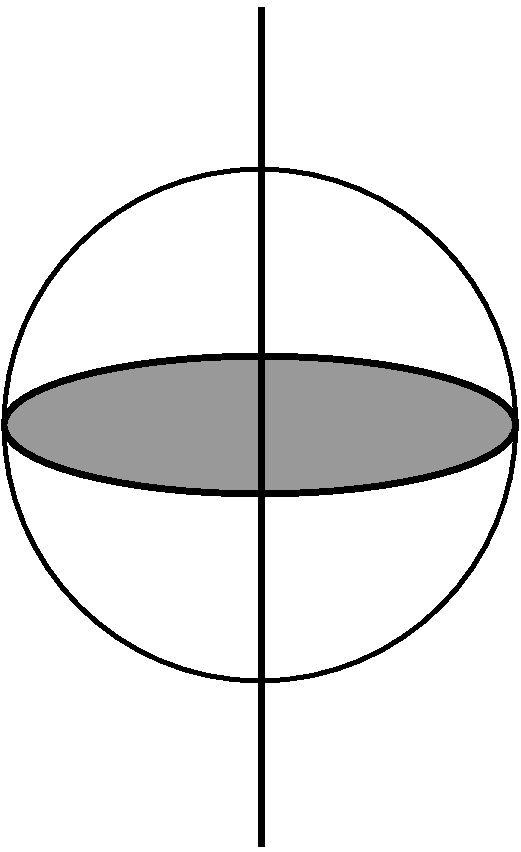
\includegraphics[height=1in]{sphere_circle_line}\\
         \emph{Note: the line intersects the sphere and the circle at their common center point.}
      \end{center}
      \begin{enumerate}
         \item Pick a number of different types of points on this object.  Calculate LH and the associated persistence diagrams for each of your choices.  Be comprehensive, both in choice of point type and in choice of radii.\vfill
         \item 
         \begin{enumerate}
           \item Using the functions \verb|samplefromlinesegment|, \verb|spheresampler|, and \verb|samplefromball|, write a Matlab function that samples from such an object. Your code should sample from each of the three elements (line, circle, sphere) with probability $1/3$.\\
         \item Use your code to sample $500$ points from this object.  Plot the resulting point cloud to verify your code works correctly.  You will need the function $\verb|plot3|$, rather than $\verb|plot|$.\\
         \item Verify your answers above by using Matlab to compute LH and the persistence diagrams for your point choices above.\\
        \end{enumerate}
      \end{enumerate}
  \end{enumerate}
\pagebreak       
\section{Investigations with Samples and Noise} 

For each of the above examples, investigate the effect of increasing the number of sampled points, and of adding noise.  If you embed your object in a higher dimension space, then add noise of that dimension, does that change your results?  Investigate and take notes.

\label{LastPage}
\end{document}